\newpage
\pagestyle{empty}    % 清空页码                                      %
\vskip -0.3in
\begin{figure}[h!]
\centering
\hspace*{4.5in}
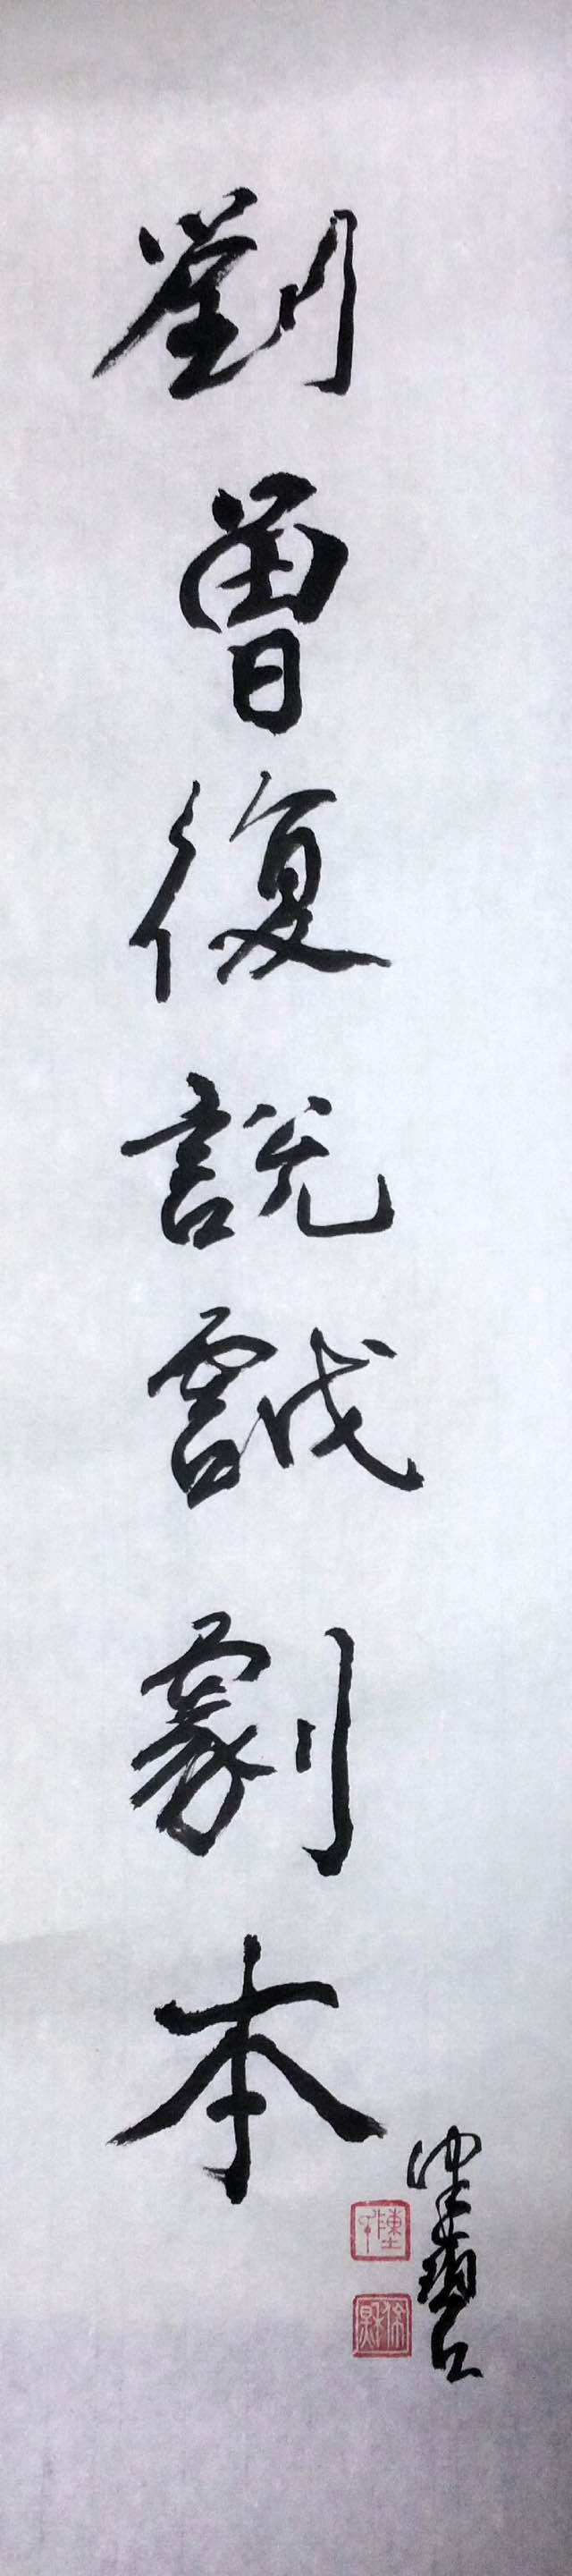
\includegraphics[height=1.30\textwidth,width=0.25\textwidth,viewport=0 0 620 2850,clip]{Figures_Peking-Opera/Liu_script-Inscription.JPG}
%\caption*{\hei 陈佩秋(谢稚柳~夫人)先生~题签}
\label{Chen-Peking_Opera_Script-Inscription-2015}
\end{figure}

\newpage
\pagestyle{empty}    % 清空页码                                      %
\begin{figure}[h!]
\centering
\vspace{+0.2in}
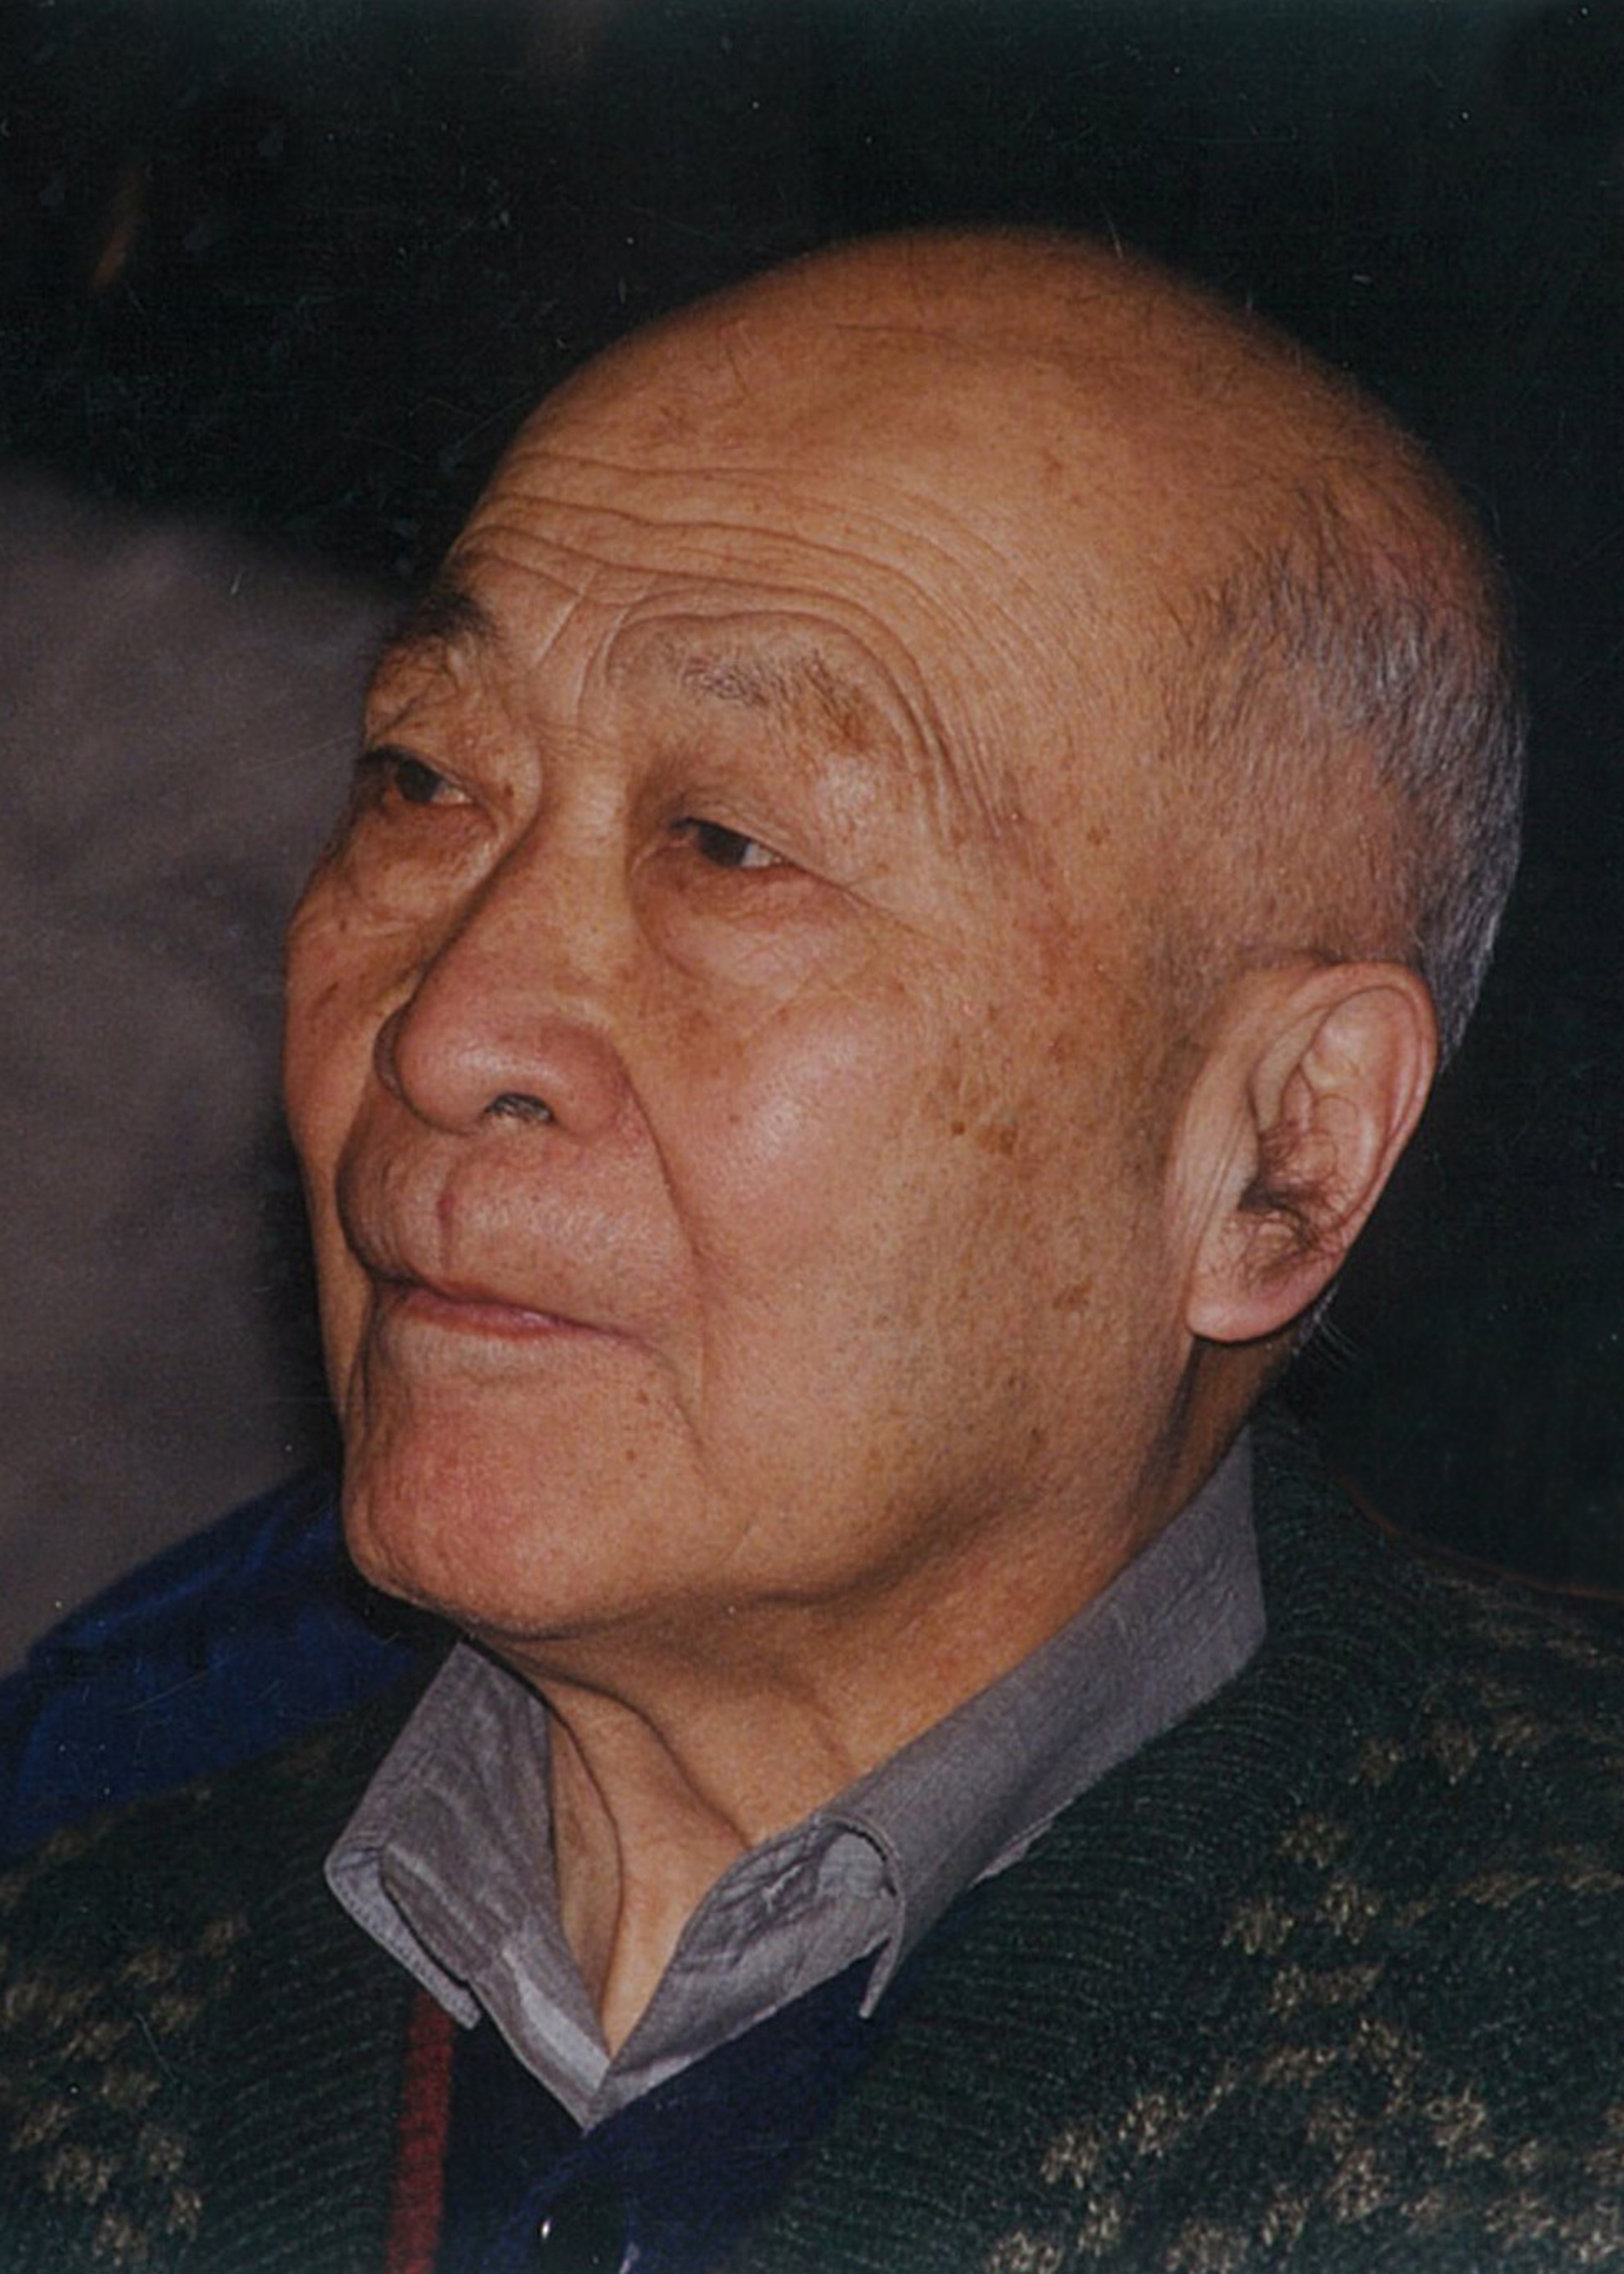
\includegraphics[height=1.20\textwidth,width=0.82\textwidth,viewport=0 0 360 520,clip]{Liu_Zengfu.jpg}
\caption*{\hei 刘曾复~教授~~(1914.11.9-2012.6.27)}
\label{Liu_Zengfu}
\end{figure}

\newpage
\begin{figure}[h!]
\centering
\vspace{-0.2in}
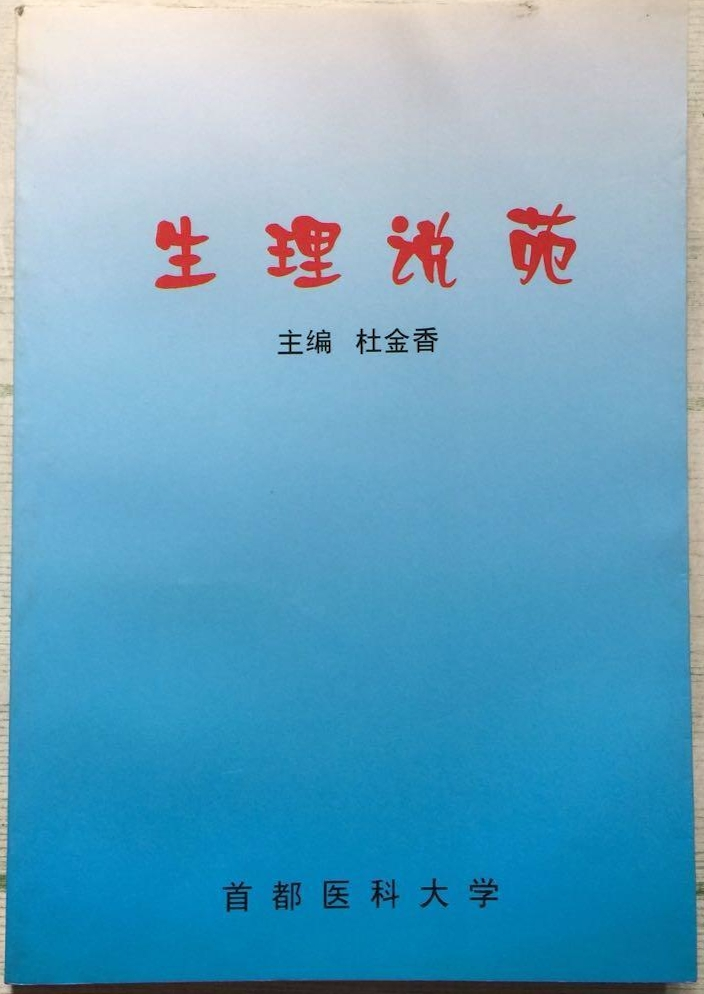
\includegraphics[height=0.65\textwidth,width=0.48\textwidth,viewport=0 0 700 1000,clip]{Liu-Physiology.jpg}
\label{Liu-Physiology}
\end{figure}
\begin{figure}[hbtp!]
\hspace*{-0.4in}
\begin{minipage}[t]{0.48\textwidth}
	\centering
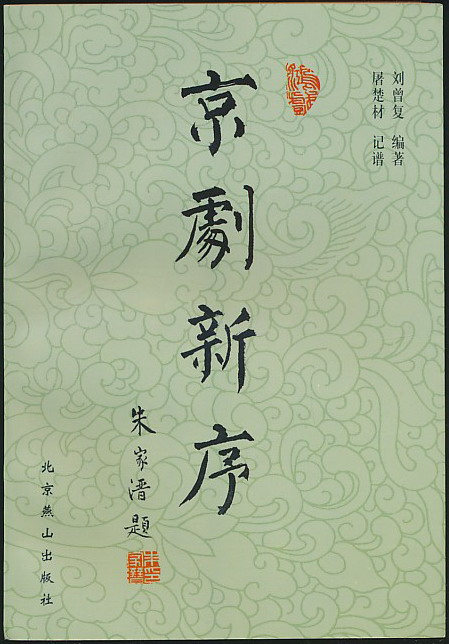
\includegraphics[height=1.50\textwidth,width=1.05\textwidth,viewport=0 0 450 650,clip]{Liu-Xinxu.jpg}
\end{minipage}
\hspace{0.3in}
\begin{minipage}[t]{0.48\textwidth}
	\centering
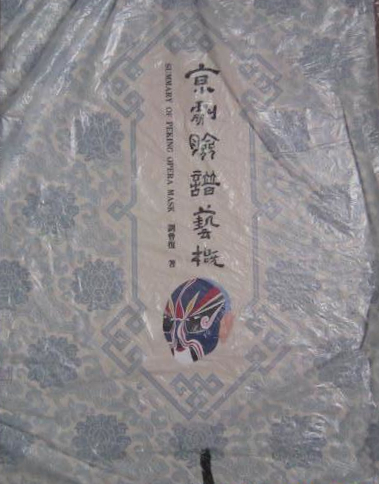
\includegraphics[height=1.50\textwidth,width=1.25\textwidth,viewport=0 0 410 490,clip]{Liu-Mask.jpg}
\end{minipage}
\vspace{1.0pt}
\caption*{\hei 刘曾复~教授~主要代表著作}
\label{Major_Works}
\end{figure}

\newpage
\begin{figure}[h!]
\centering
%\vspace{+0.2in}
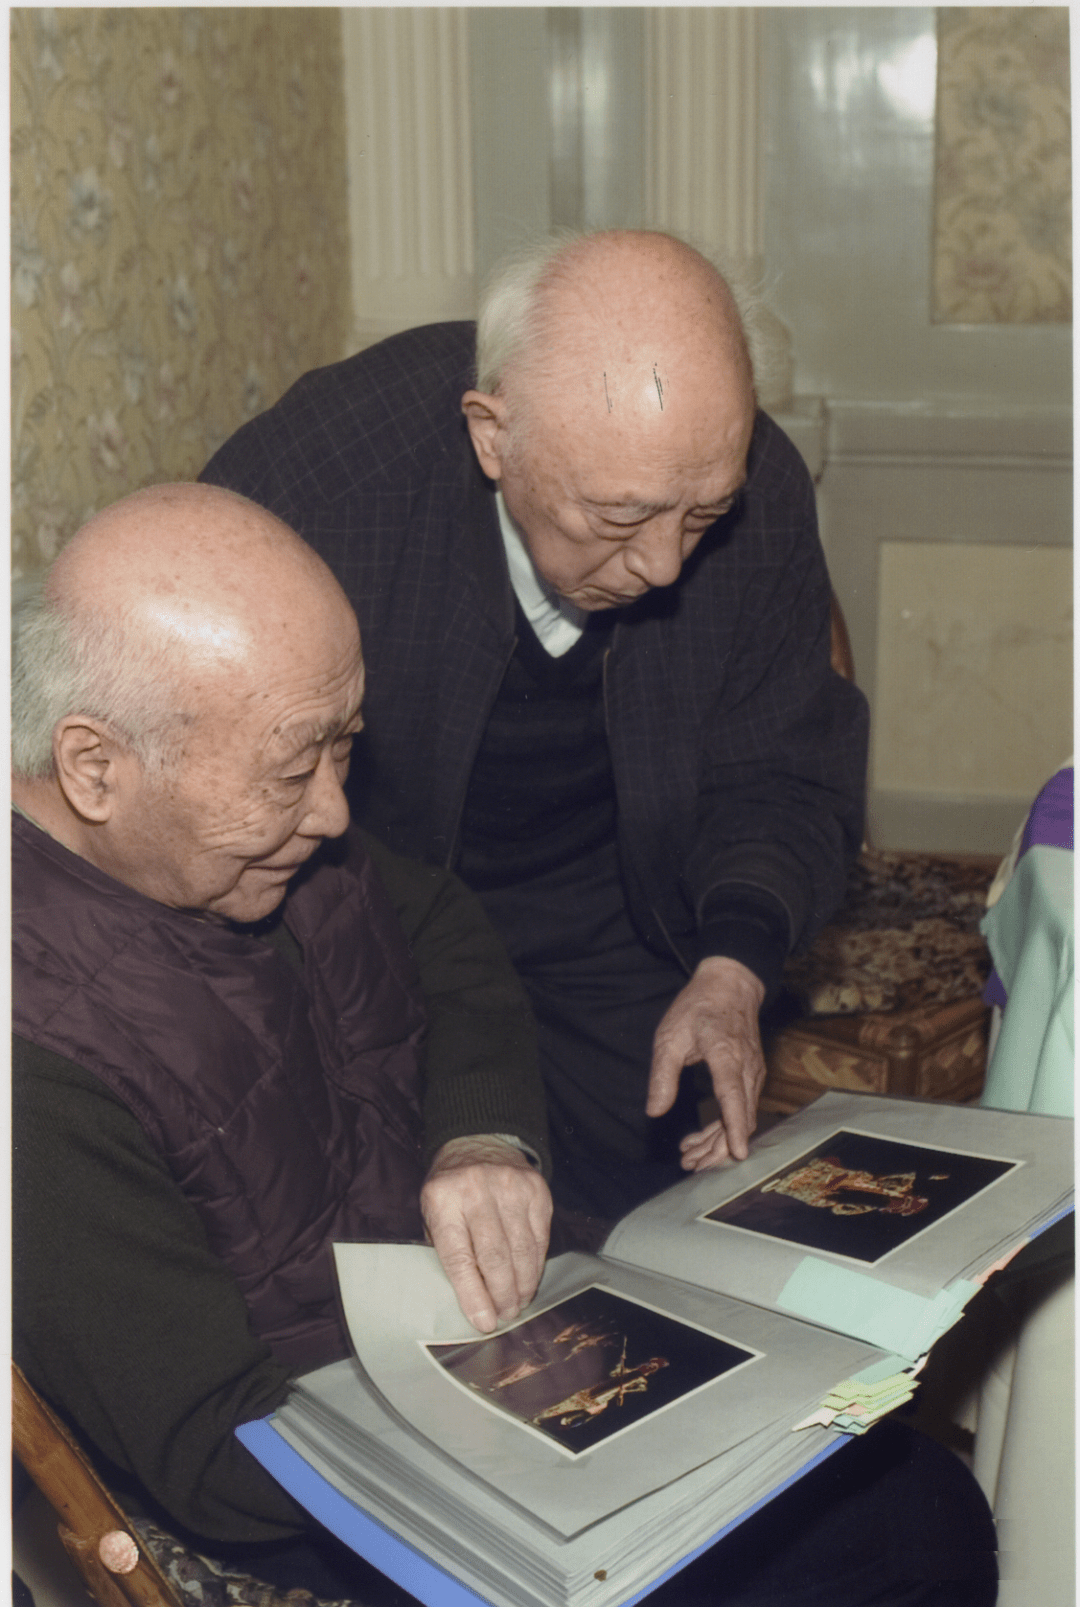
\includegraphics[height=1.38\textwidth,width=1.0\textwidth,viewport=0 0 1050 1550,clip]{Liu-Wu.png}
\caption*{\hei 刘曾复~先生~和~吴小如~先生}
\label{Collect_Liu_Wu}
\end{figure}

\newpage
\begin{figure}[h!]
\centering
%\vspace{-10.5pt}
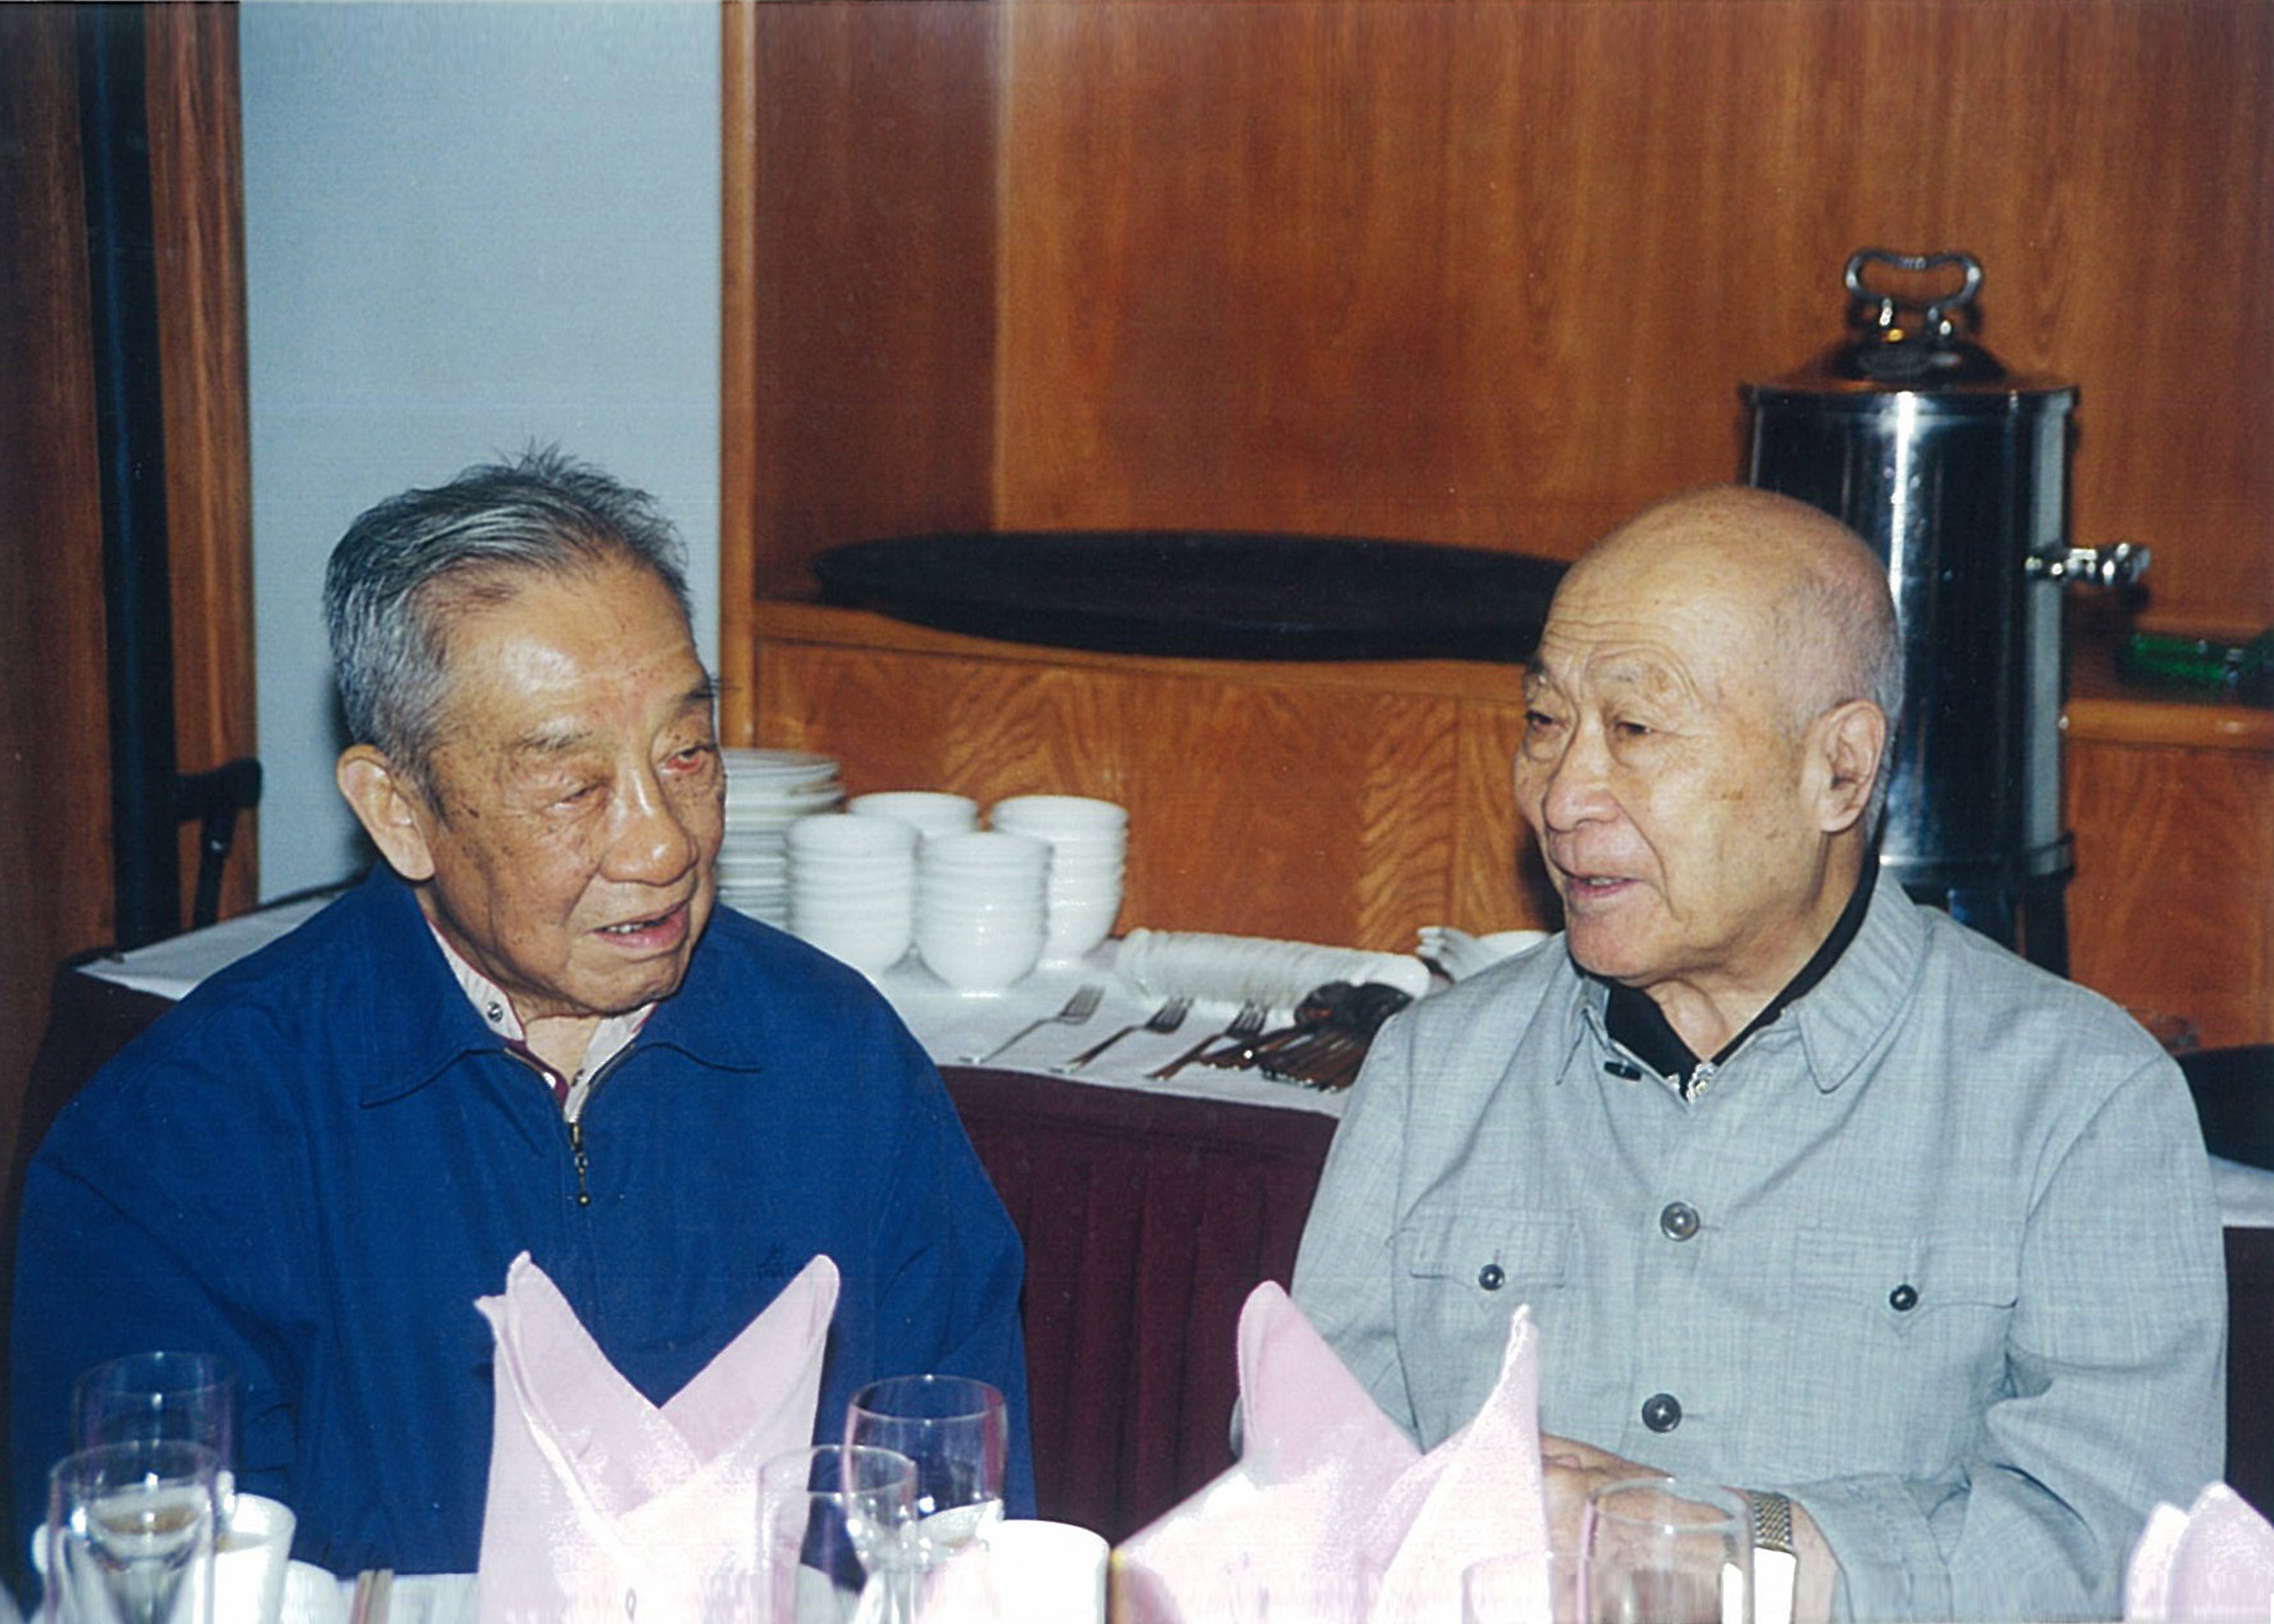
\includegraphics[height=0.60\textwidth,width=1.0\textwidth,viewport=0 0 500 300,clip]{Zhu-Liu.jpg}
\caption*{\hei 朱家溍~先生~和~刘曾复~先生}
\label{Collect_Zhu_Wu}
\end{figure}

\begin{figure}[h!]
\centering
%\vspace{-10.5pt}
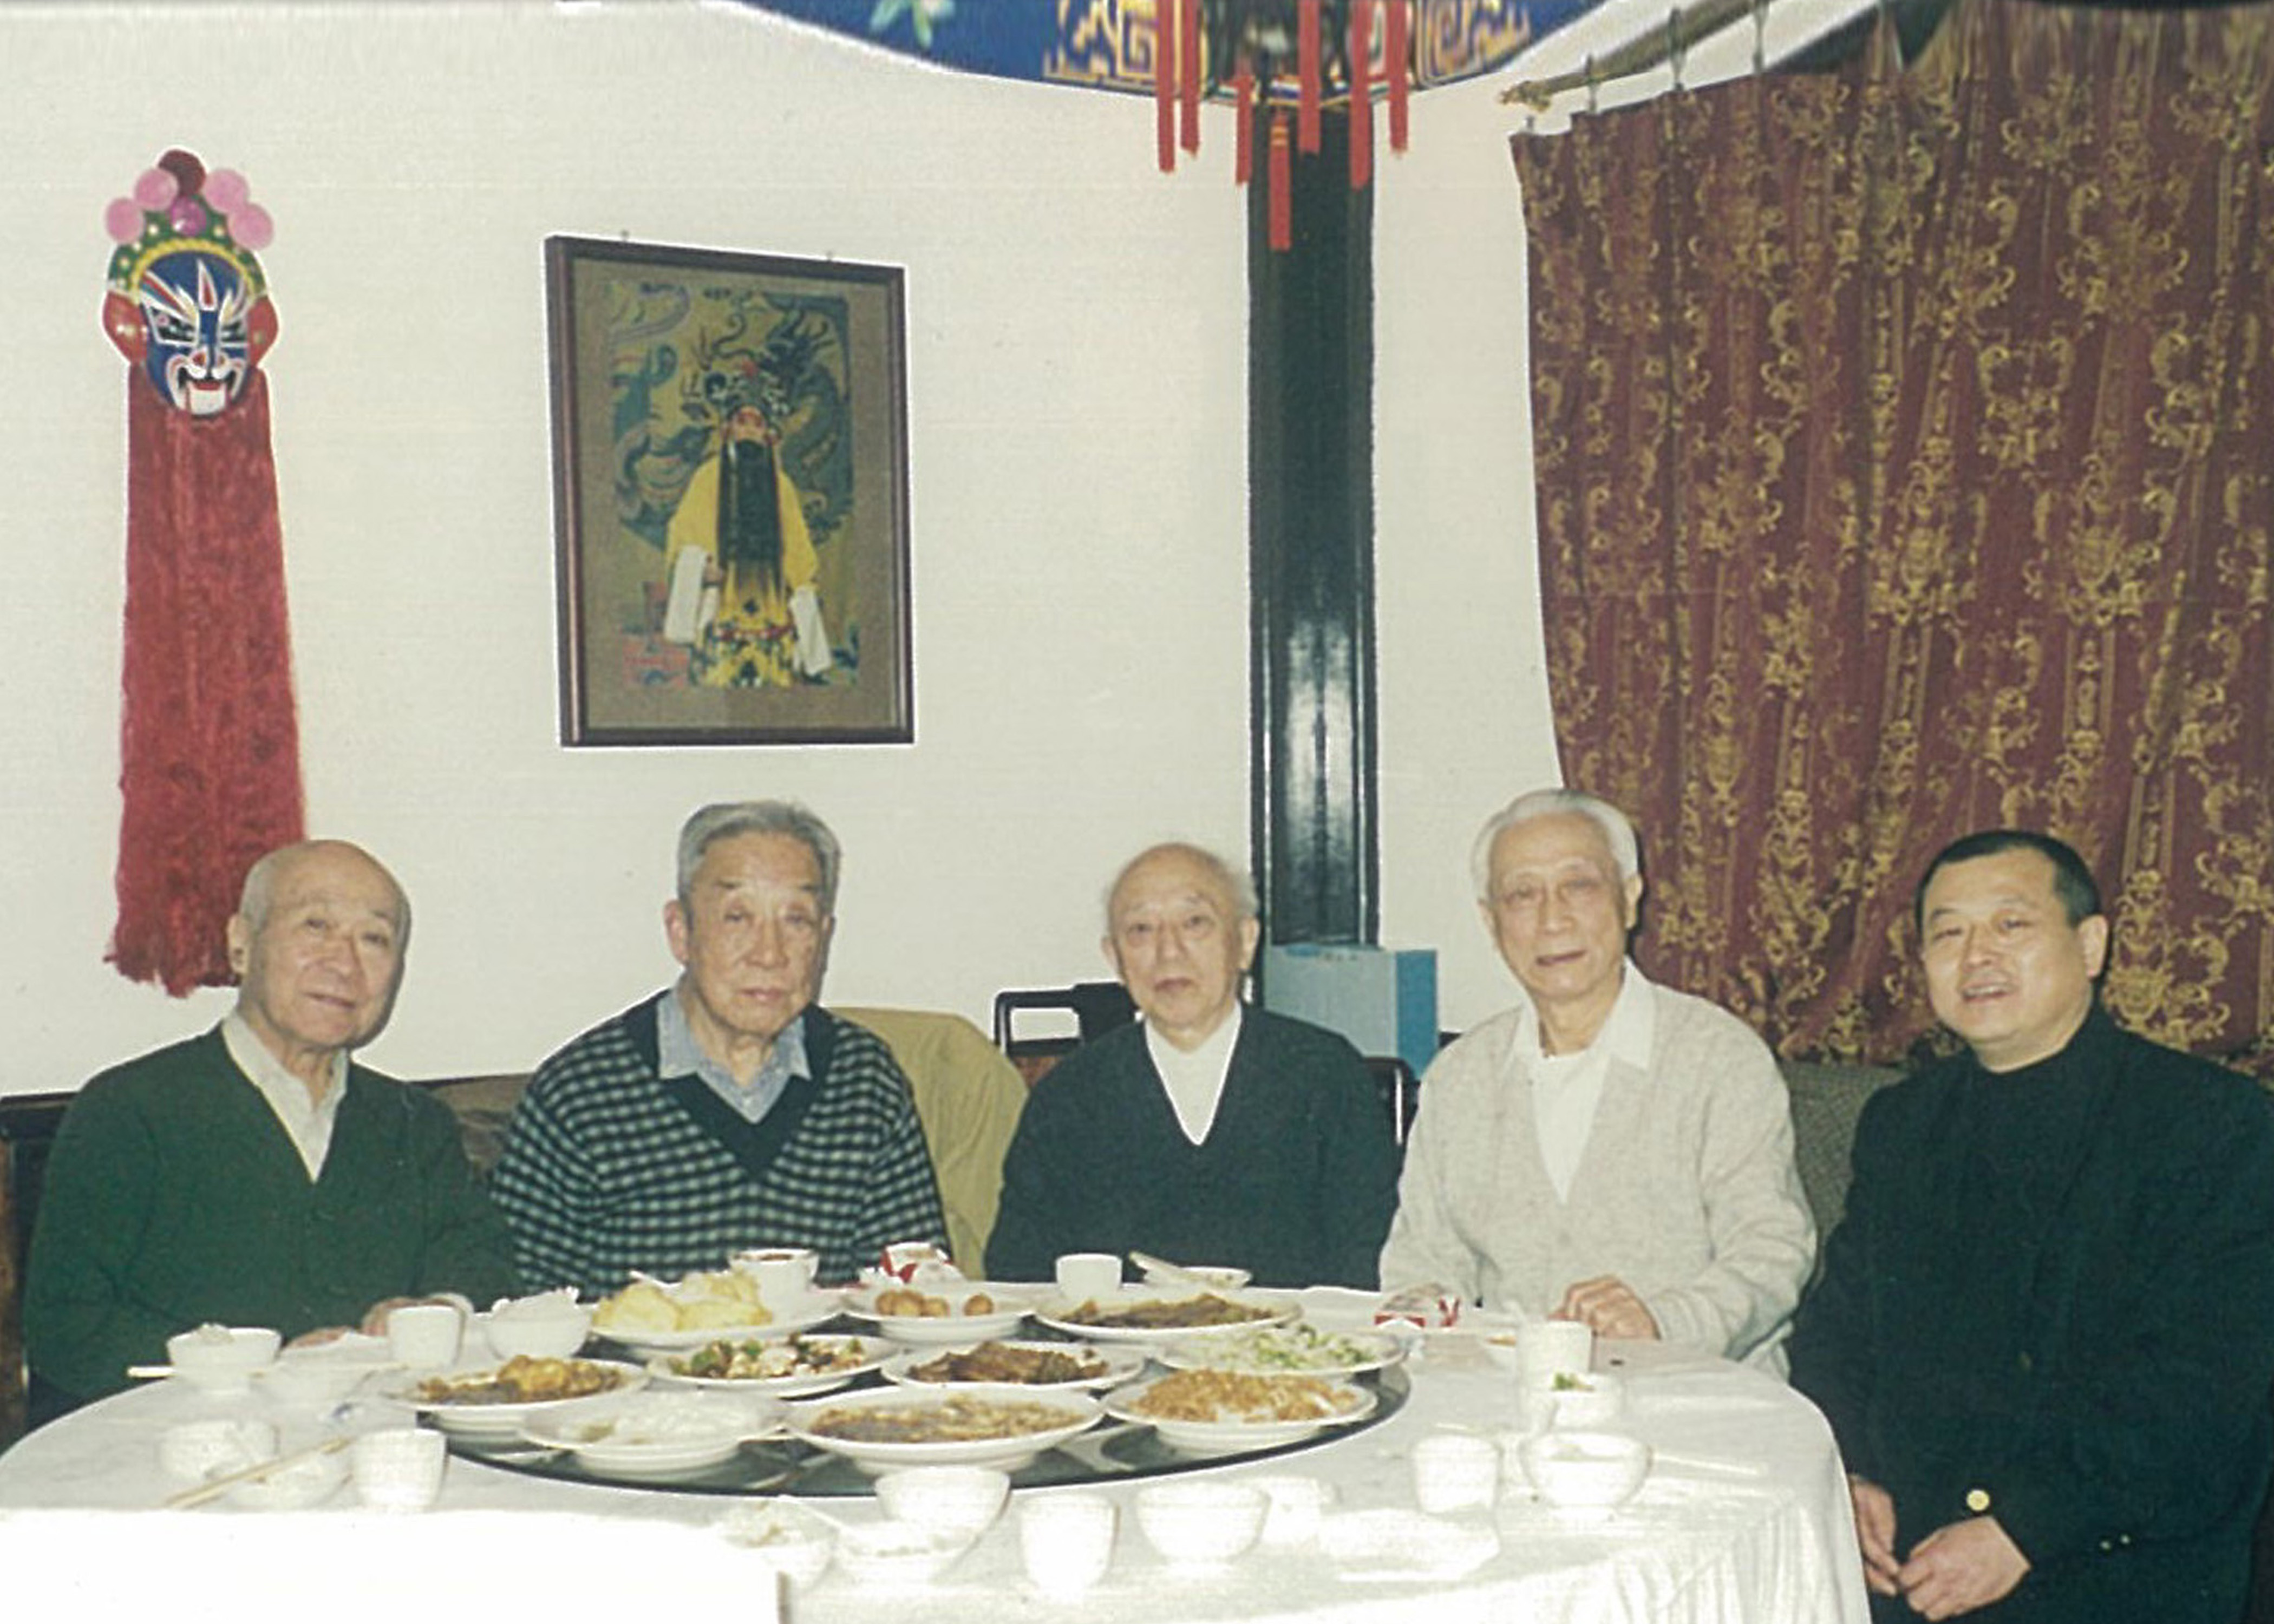
\includegraphics[height=0.60\textwidth,width=1.0\textwidth,viewport=0 0 500 300,clip]{Collect_Zhu-Liu-Wu-Wang.jpg}
\caption*{\hei 左起:~刘曾复~先生、朱家溍~先生、吴小如~先生、王金璐~先生~等~合影}
\label{Collect_Liy_Zhu_Wu_Wang}
\end{figure}

\newpage
\begin{figure}[h!]
\centering
\vspace{-0.6in}
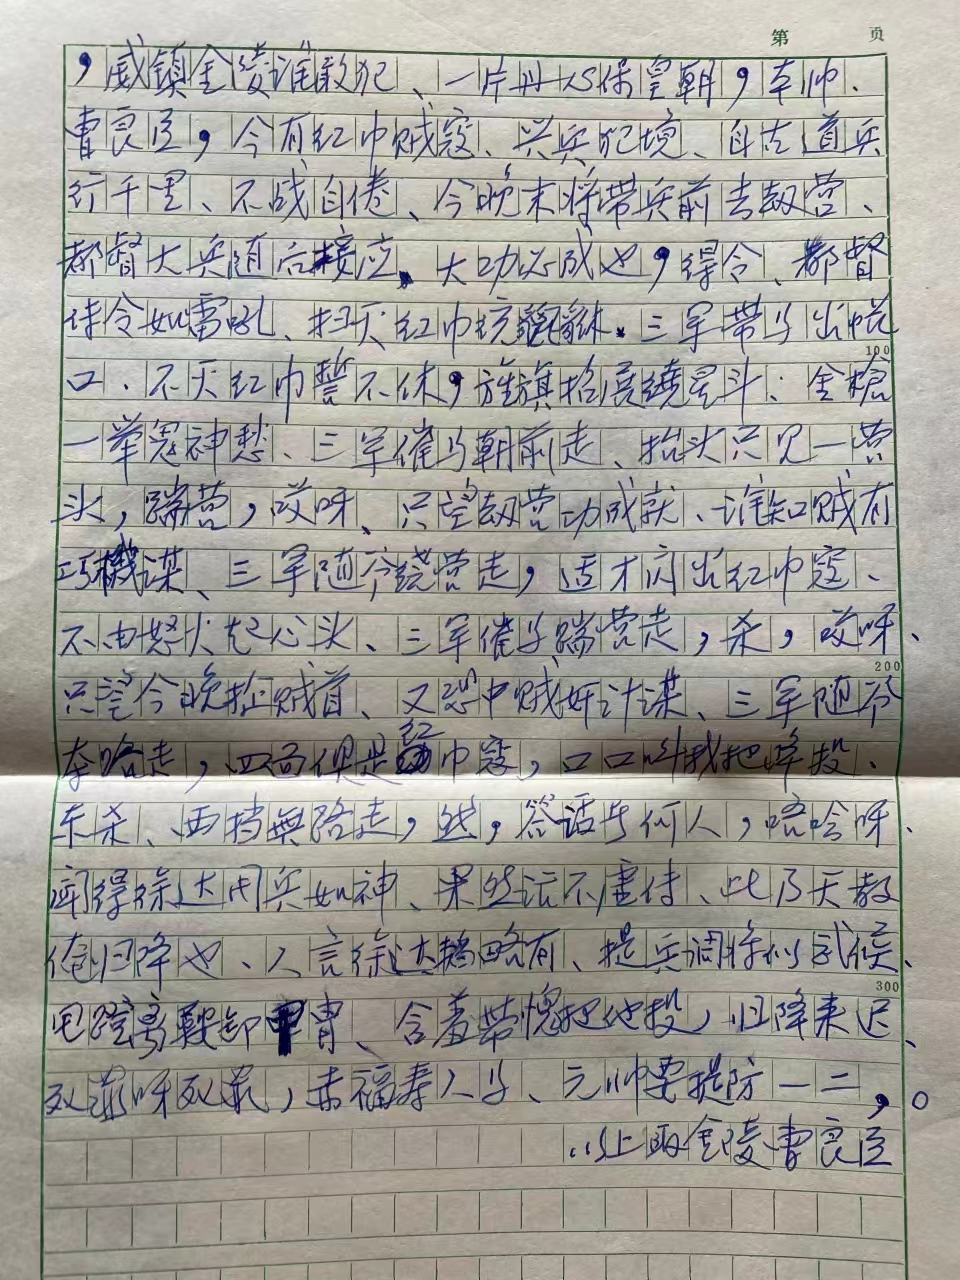
\includegraphics[height=0.68\textwidth,width=0.50\textwidth,viewport=0 0 950 1300,clip]{PekOpe_Liu-1.jpg}
\caption*{\hei 刘曾复~先生~抄录的《取金陵》曹良臣的单词}
\label{Liu-Script}
\end{figure}
\vspace{30pt}
\begin{figure}[hbtp!]
\hspace*{-0.5in}
\begin{minipage}[t]{0.53\textwidth}
	\centering
	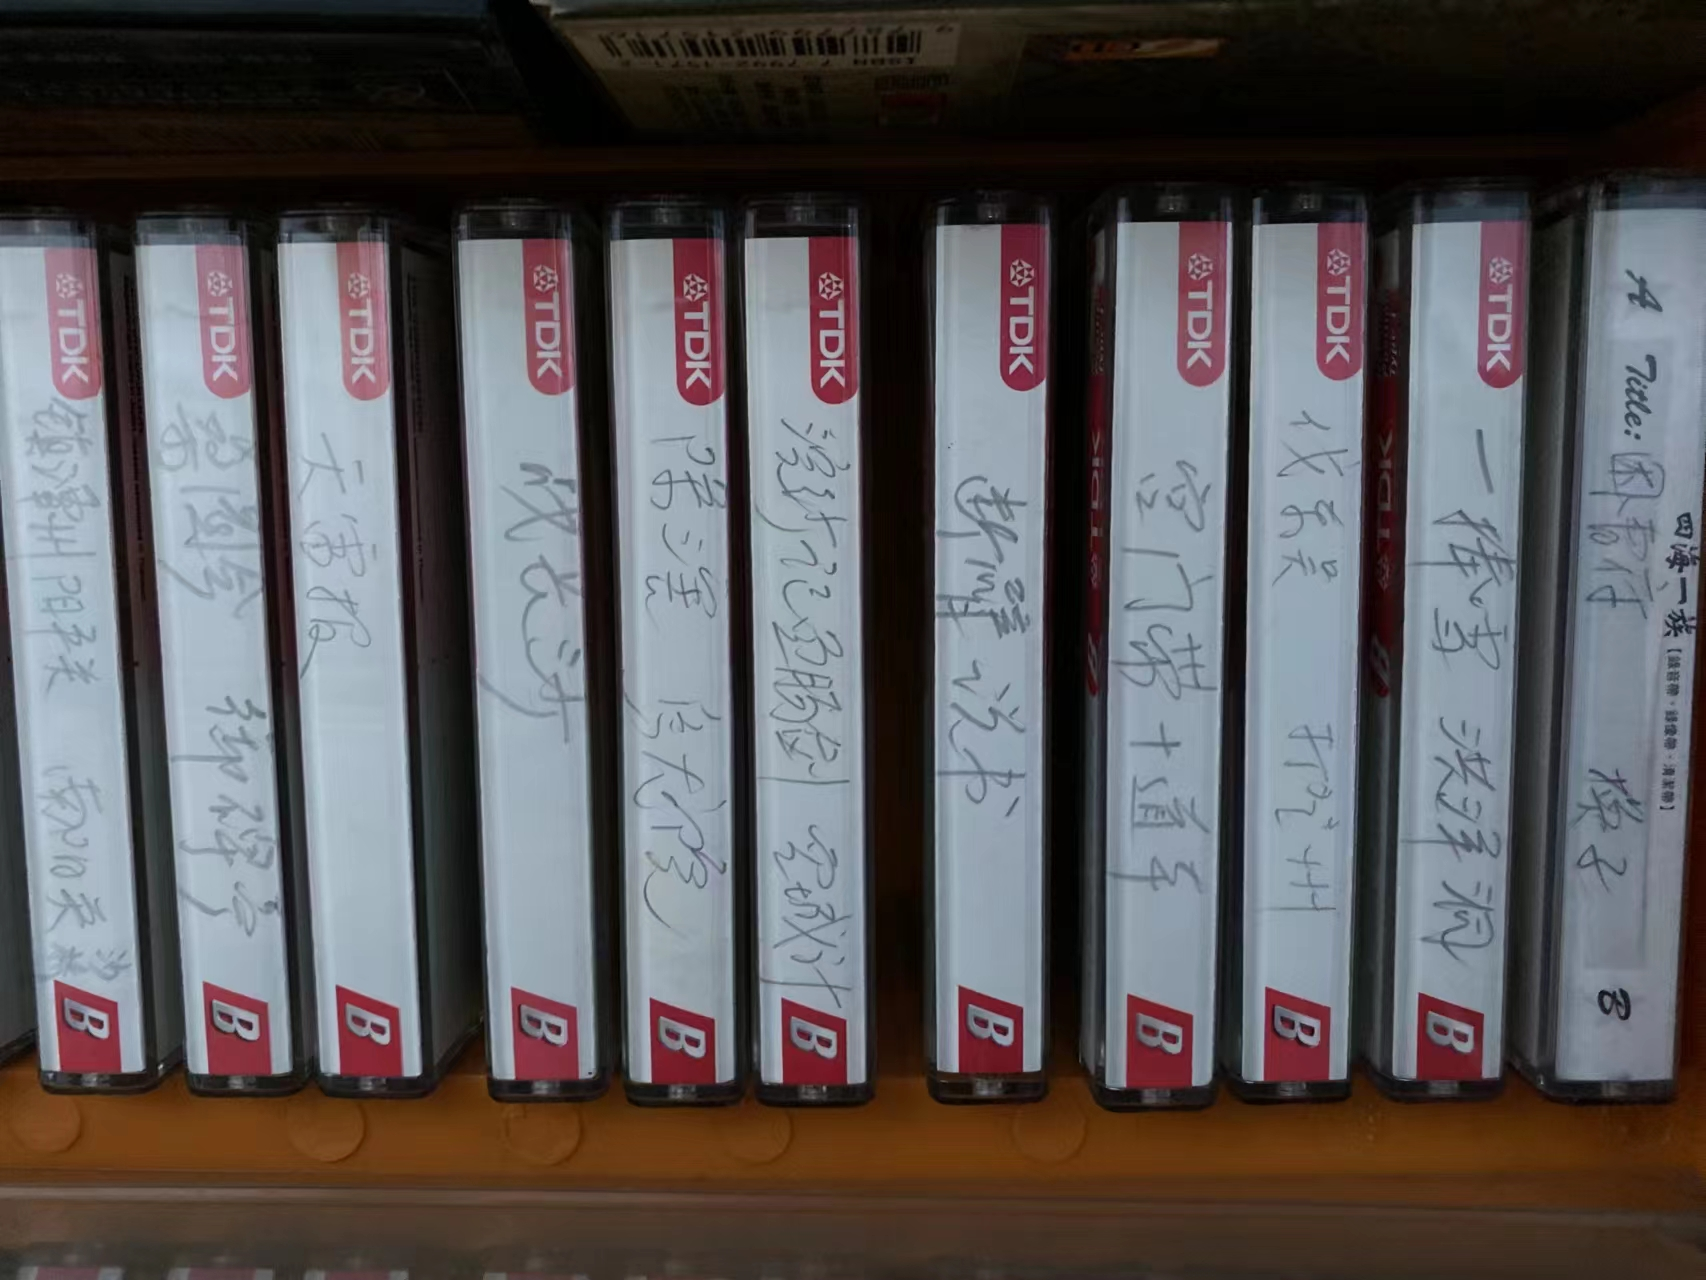
\includegraphics[height=1.00\textwidth,width=1.20\textwidth,viewport=0 0 1750 1300,clip]{PekOpe_Liu-2.jpg}
	\caption*{\hei \fontsize{8.5pt}{4.0pt}\selectfont{左:~刘曾复~先生~保存的部分说戏录音磁带}}
\end{minipage}
\hspace{0.6in}
\begin{minipage}[t]{0.43\textwidth}
	\centering
	\vspace{-3.7in}
	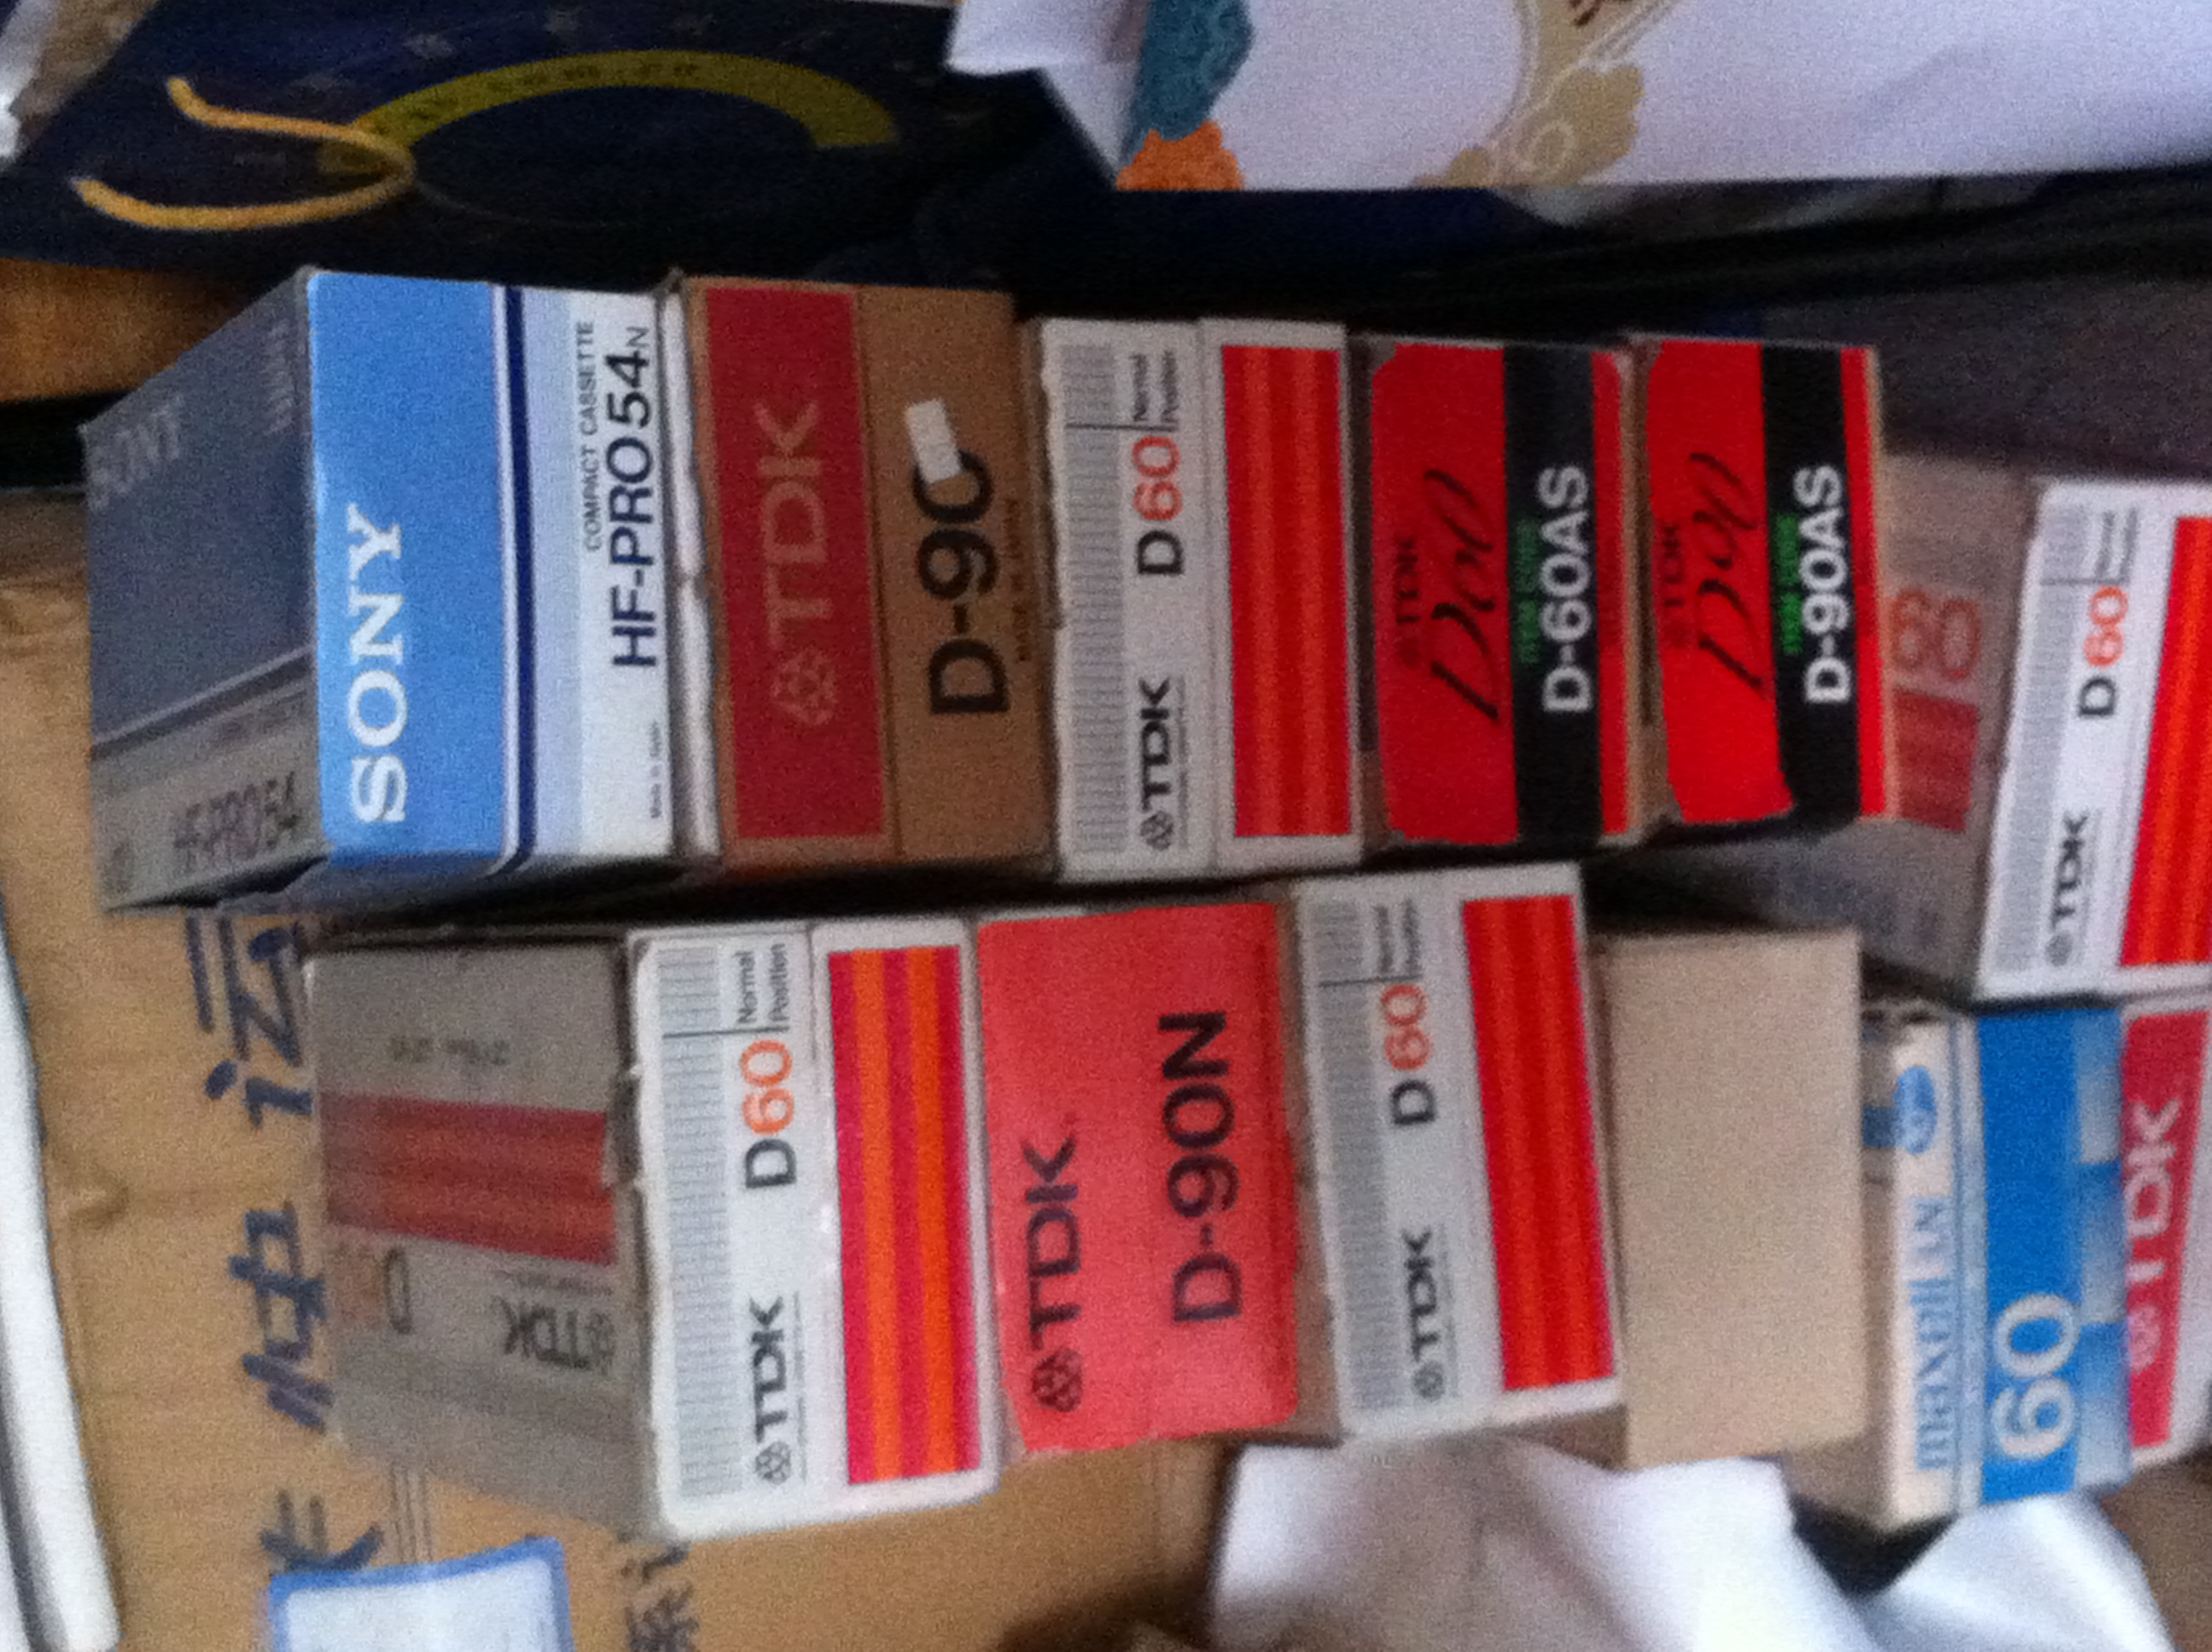
\includegraphics[height=1.10\textwidth,width=1.70\textwidth,angle=270, viewport=0 0 2750 1950,clip]{PekOpe_Wu-5.jpg}
%	\caption*{\hei \fontsize{8.5pt}{4.0pt}\selectfont{右:吴小如~先生~保存的刘曾复先生的说戏录音磁带}}
	\caption*{\hei \fontsize{8.5pt}{4.0pt}\selectfont{右:吴小如~先生~保存的各类说戏录音磁带}}
\end{minipage}
\label{Records}
\end{figure}
\newpage
\begin{figure}[h!]
\centering
\vspace{-0.6in}
	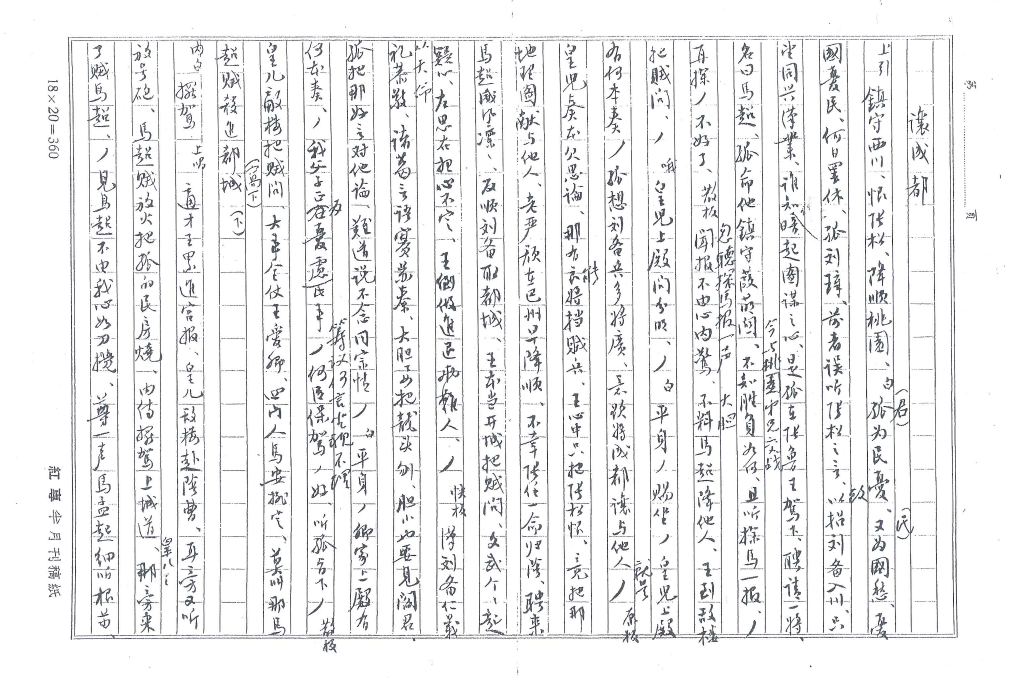
\includegraphics[height=0.50\textwidth,width=0.78\textwidth,viewport=0 0 750 470,clip]{PekOpe_Wu-script-1.png}
	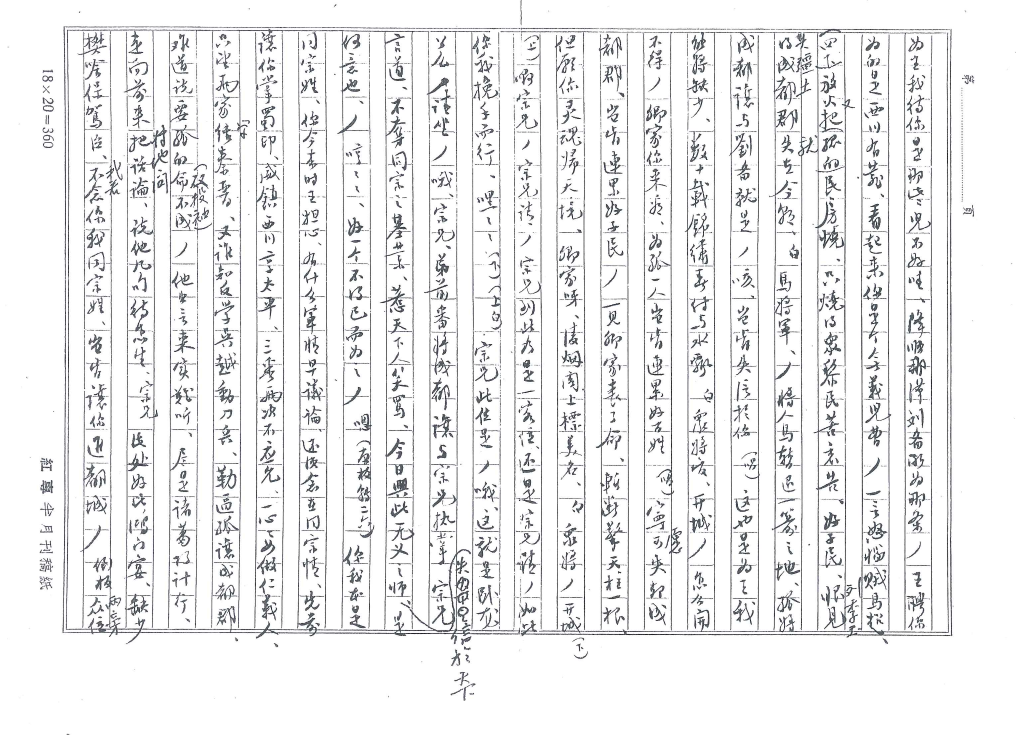
\includegraphics[height=0.50\textwidth,width=0.81\textwidth,viewport=0 0 750 520,clip]{PekOpe_Wu-script-2.png}
	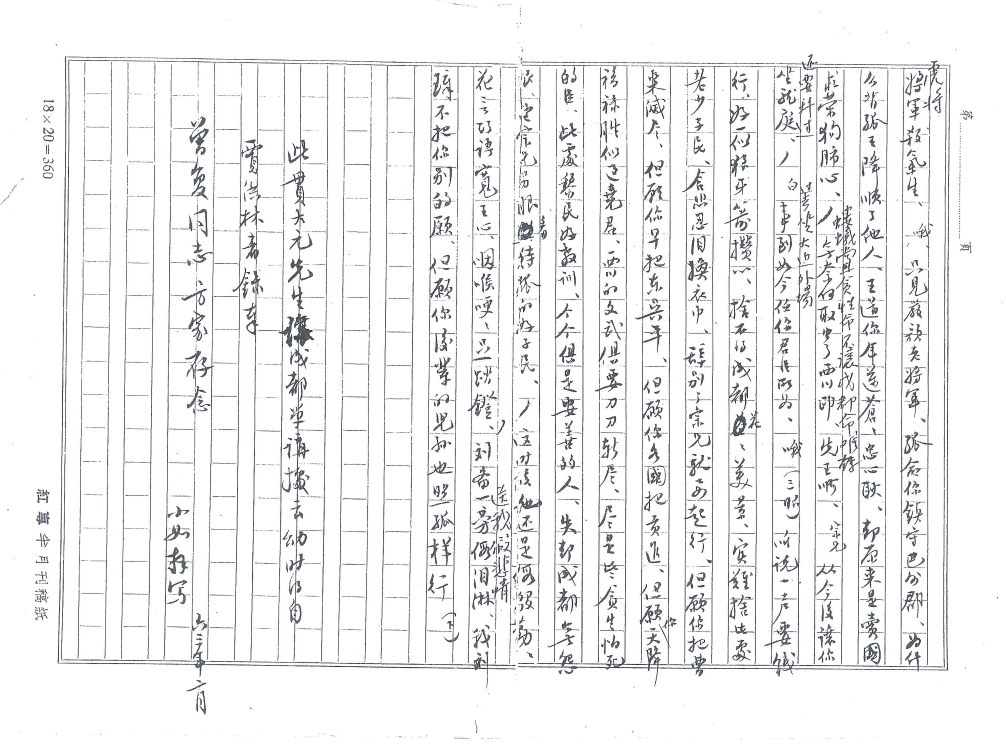
\includegraphics[height=0.50\textwidth,width=0.8\textwidth,viewport=0 0 750 500,clip]{PekOpe_Wu-script-3.png}
%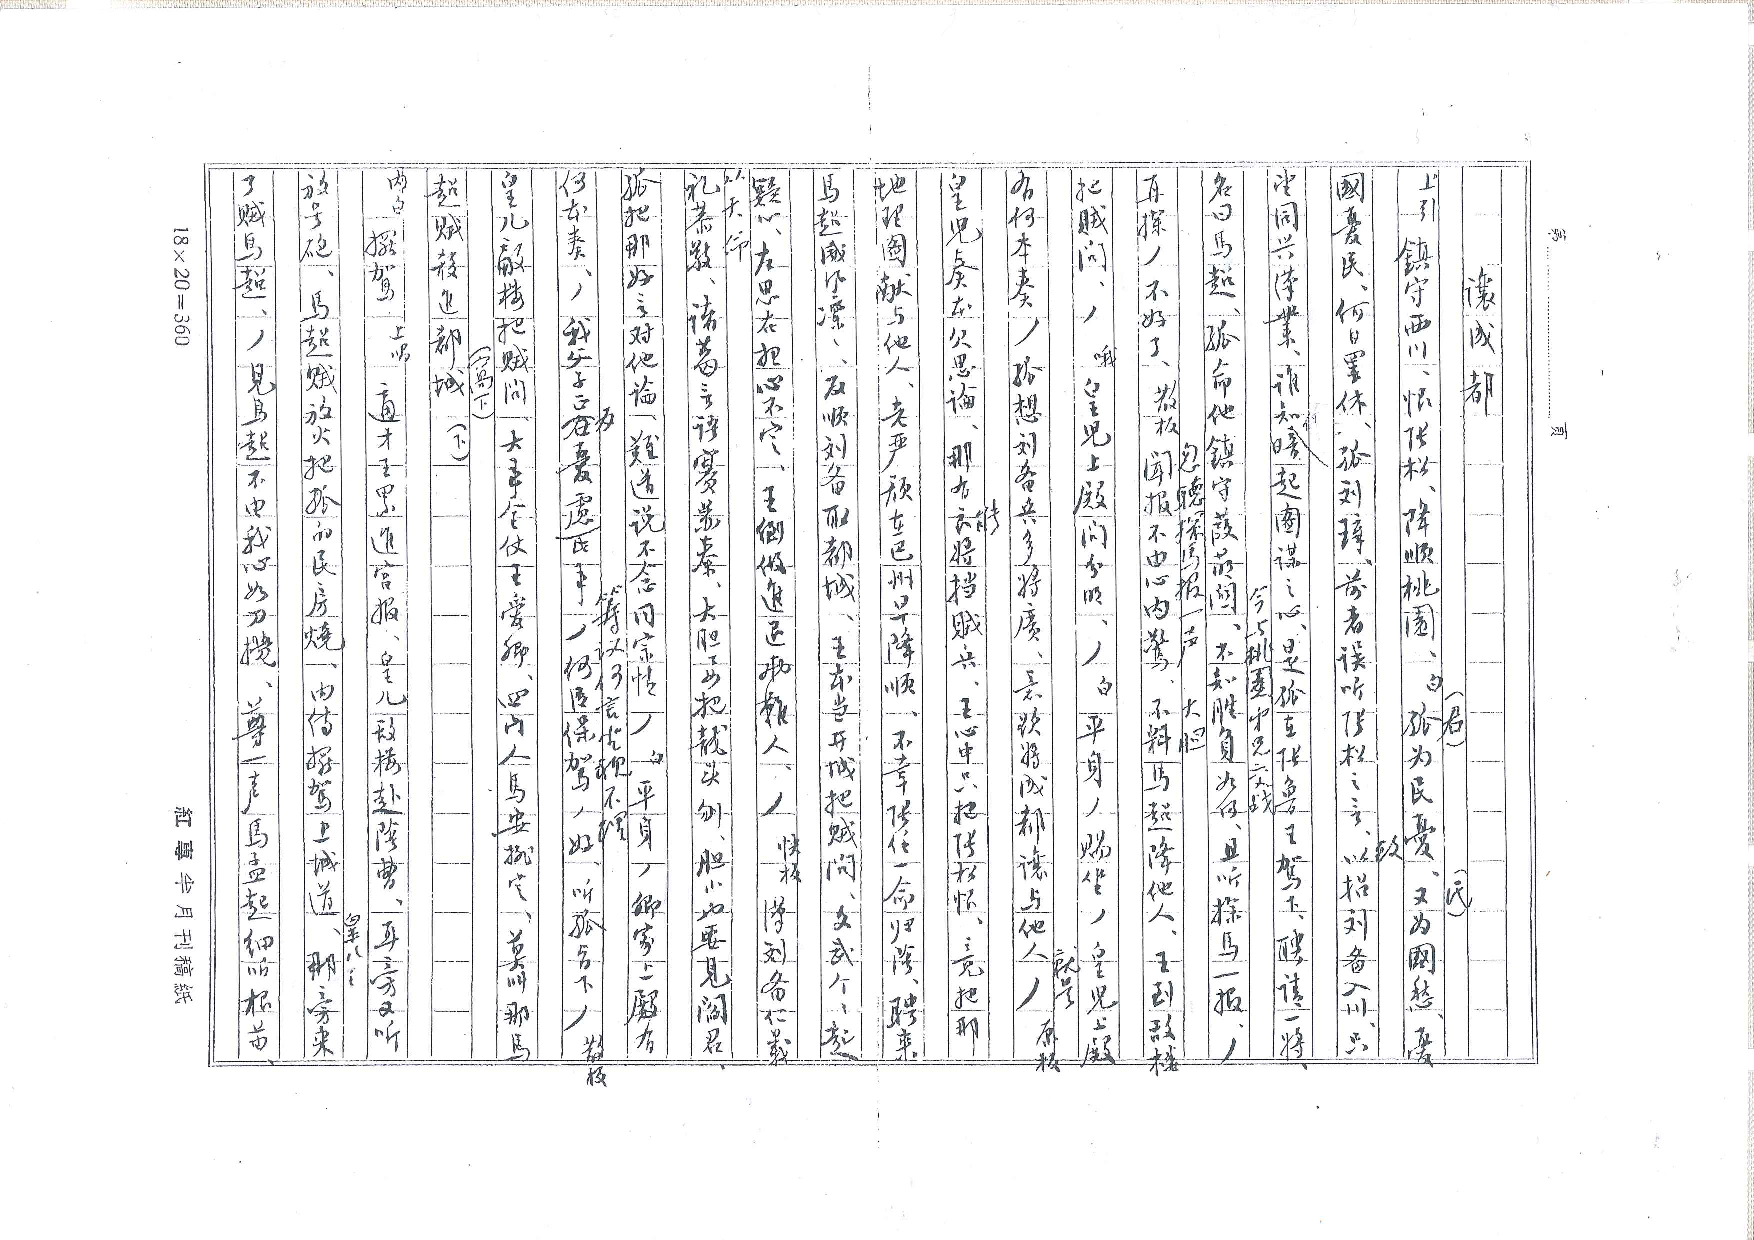
\includepdf[fitpaper]{PekOpe_Wu-script.pdf}
\caption*{\hei 吴小如~先生~抄录的~《让成都》刘璋的单词(贯大元~先生~传)复印件,刘曾复~先生~作了修改}
\label{Wu-Script}
\end{figure}

\newpage
\begin{figure}[h!]
\centering
%\vspace{-10.5pt}
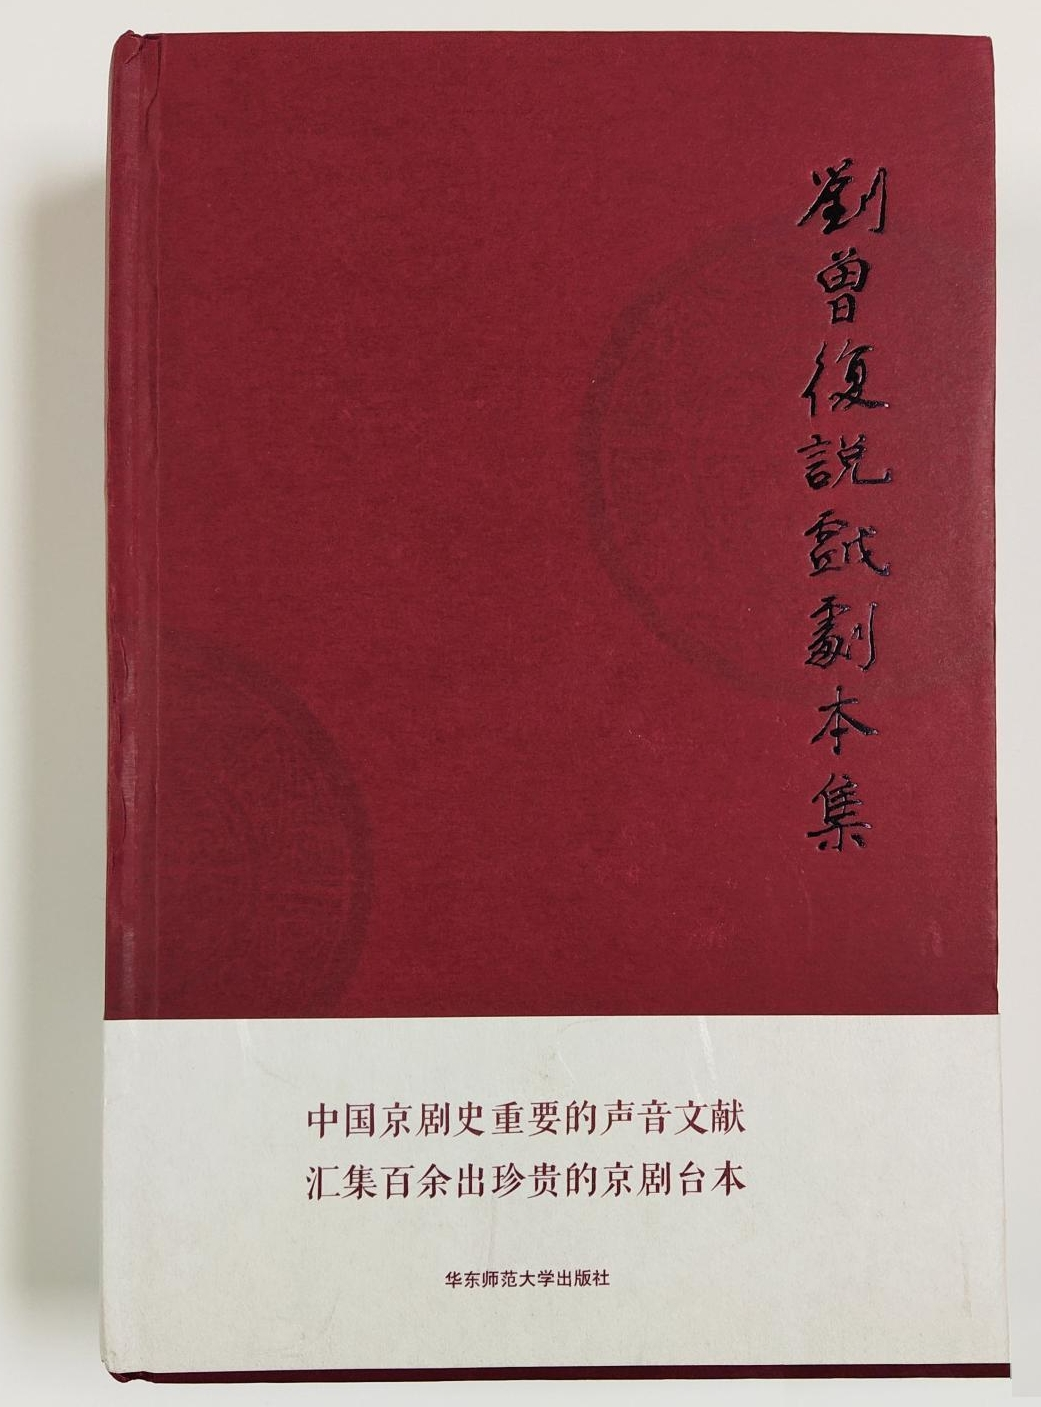
\includegraphics[height=1.30\textwidth,width=1.02\textwidth,viewport=0 0 1030 1400,clip]{Figures_Peking-Opera/Liu_script.jpg}
\caption*{\hei \fontsize{8.5pt}{4.0pt}\selectfont{《刘曾复说戏剧本集》初版~(上海~华东师范大学出版社~2015.08)~书影}}
\label{Peking_Opera_Script}
\end{figure}
%\keywords{Keyword1; Keyword2; Keyword3}

